\documentclass[12pt]{article}
\usepackage{graphicx}
\usepackage{amsmath}
\usepackage{listings}
\lstset{language=Matlab, basicstyle=\ttfamily}
\usepackage{geometry} % Required for customizing margins

\geometry{margin=1in} % Sets 1-inch margins on all sides

\title{ELCT 432 Computer Assignment \#3}
\author{Jacob C. Vaught}
\date{}

\begin{document}

\maketitle

\section*{Introduction}
This report aims to analyze different modulation schemes, taking into account both theoretical and practical aspects. We will be looking at the signal \(u(t)\) in different scenarios, its bandwidth, and its complex low-pass equivalent.

\section*{Case A: Transmitted Signal with Frequency Modulation}
\subsection*{Expression for \(u(t)\)}
For this scenario, the transmitted signal \(u(t)\) is given by:
\[
u(t) = \cos(2\pi (f_c + f_m) t)
\]
where \(f_c = 915 \text{ MHz}\) and \(f_m = 200 \text{ kHz}\).

\subsubsection*{MATLAB Code}
\begin{lstlisting}
% Parameters
fsample = 2e6; % Fixed at the SDRs
fc = 915e6; % Carrier frequency
fm = 200e3; % Modulating frequency
Nsamples = 40000; % Number of samples
time = [0:Nsamples-1]' * 1/fsample;

% Generate the signal
IQdataTX = cos(2*pi*(fc + fm)*time);
\end{lstlisting}

\subsection*{Theoretical Bandwidth Calculation}
The bandwidth of the transmitted signal would be twice the frequency of the modulating signal, \(2f_m\), which is \(400 \text{ kHz}\).

\subsection*{Complex Low-Pass Equivalent}
\[
u_{\text{lp}}(t) = e^{j2\pi (f_c + f_m) t}
\]
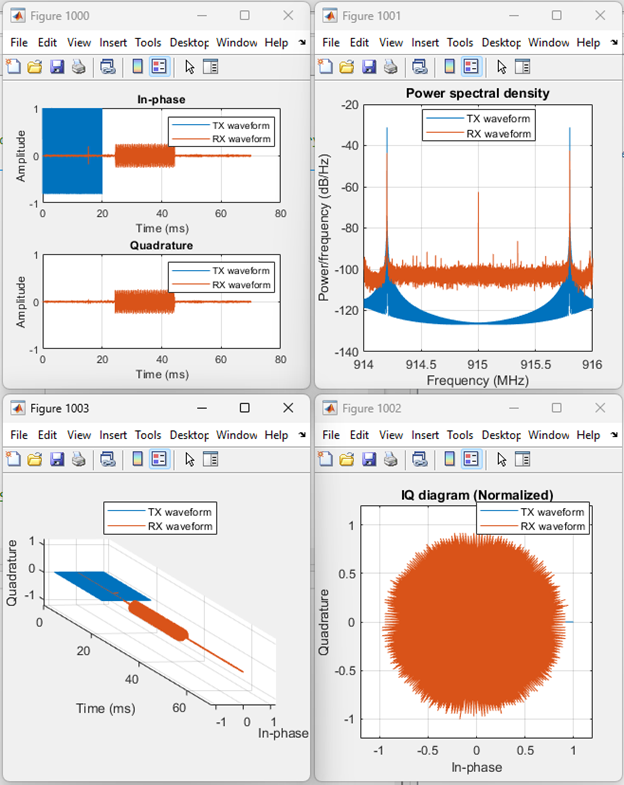
\includegraphics[width=\linewidth]{CA3_1_a.png}

\subsubsection*{Discussion}
Observations from the MATLAB plots reveal an oscillating sinusoidal signal in both the in-phase and quadrature components. The power spectral density (PSD) displays peaks at two distinct frequencies centered around 915 MHz. Unexpectedly, the bandwidth calculated from the PSD is 1.6 MHz.

\subsubsection*{Theoretical vs. Practical Bandwidth}
The theoretical calculations predict a bandwidth of 400 kHz. However, the practical bandwidth observed is 1.6 MHz. One plausible explanation for this discrepancy could be the sampling rate of 2 MHz. Subtracting the predicted bandwidth of 400 kHz from the sampling rate provides a figure close to the observed 1.6 MHz bandwidth, although further investigation would be needed to confirm this.


\section*{Case B: DSB-SC AM Signal with Cosine Message}
\subsection*{Expression for \(u(t)\)}
For this case, the message signal \(m(t) = \cos(2\pi f_m t)\) where \(f_m = 200 \text{ kHz}\). The DSB-SC AM signal can be expressed as:
\[
u(t) = m(t) \cdot \cos(2\pi f_c t)
\]
where \(f_c = 912.5 \text{ MHz}\).

\subsubsection*{MATLAB Code}
\begin{lstlisting}
% Parameters
fsample = 2e6; % Fixed at the SDRs
fc = 912.5e6; % Carrier frequency
fm = 200e3; % Modulating frequency
Nsamples = 40000; % Number of samples
time = [0:Nsamples-1]' * 1/fsample;

% Generate the signal
IQdataTX = cos(2*pi*fm*time) .* cos(2*pi*fc*time);
\end{lstlisting}

\subsection*{Theoretical Bandwidth Calculation}
The DSB-SC AM signal typically has a bandwidth of \(2f_m\), which would be \(400 \text{ kHz}\) in this case.

\subsection*{Complex Low-Pass Equivalent}
\[
u_{\text{lp}}(t) = e^{j2\pi f_m t} \cdot e^{j2\pi f_c t}
\]
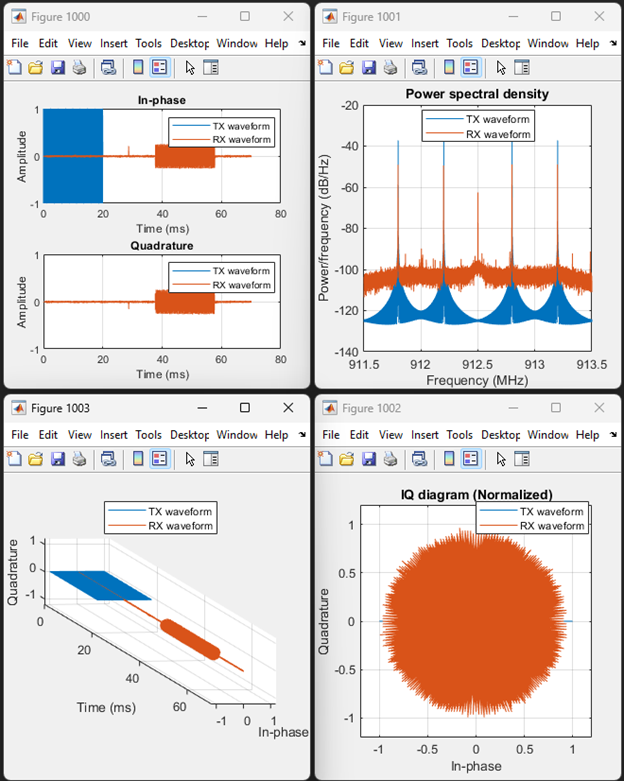
\includegraphics[width=\linewidth]{CA3_1_b.png}

\subsubsection*{Discussion}
The MATLAB plots display four distinct poles in the power spectral density (PSD). The inner two poles exhibit a bandwidth of 0.6 MHz, whereas the outer two poles have a bandwidth of 1.4 MHz. 

\subsubsection*{Theoretical vs. Practical Bandwidth}
The theoretically calculated bandwidth is 400 kHz, contrasting with the observed bandwidths in the PSD. The presence of four poles suggests that additional spectral components are involved, possibly due to the method of generation or characteristics inherent to DSB-SC AM. Further investigation is required to reconcile these differences.


\section*{Case C: Conventional AM Signal with Cosine Message}
\subsection*{Expression for \(u(t)\)}
In this case, the message signal \(m(t) = \cos(2\pi f_m t)\) with \(f_m = 200 \text{ kHz}\). The conventional AM signal \(u(t)\) can be expressed as:
\[
u(t) = (1 + a \cdot m(t)) \cdot \cos(2\pi f_c t)
\]
where \(f_c = 912 \text{ MHz}\) and \(a = 0.5\).

\subsubsection*{MATLAB Code}
\begin{lstlisting}
% Parameters
fsample = 2e6; % Fixed at the SDRs
fc = 912e6; % Carrier frequency
fm = 200e3; % Modulating frequency
a = 0.5; % Modulation index
Nsamples = 40000; % Number of samples
time = [0:Nsamples-1]' * 1/fsample;

% Generate the signal
IQdataTX = (1 + a * cos(2*pi*fm*time)) .* cos(2*pi*fc*time);
\end{lstlisting}

\subsection*{Theoretical Bandwidth Calculation}
The bandwidth for conventional AM signals is \(2f_m\), which equates to \(400 \text{ kHz}\) in this instance.

\subsection*{Complex Low-Pass Equivalent}
\[
u_{\text{lp}}(t) = (1 + a \cdot e^{j2\pi f_m t}) \cdot e^{j2\pi f_c t}
\]
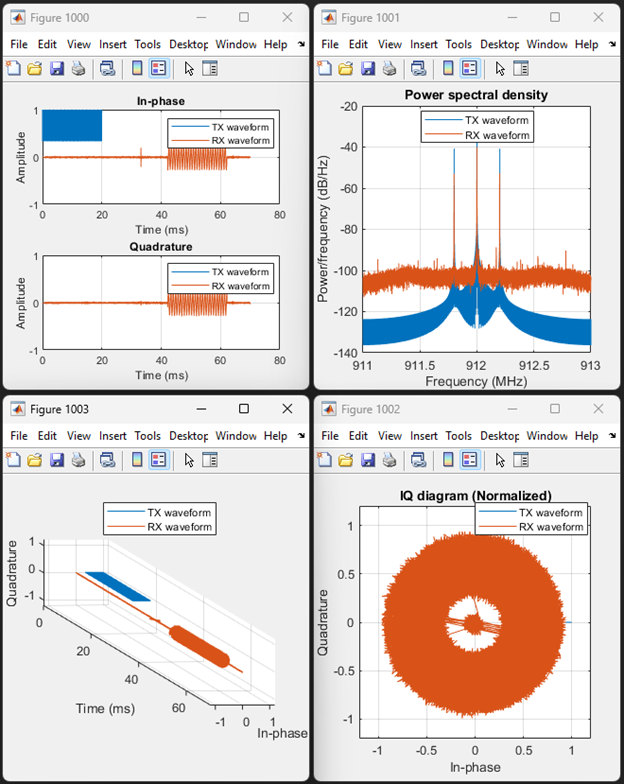
\includegraphics[width=\linewidth]{CA3_1_c.png}

\subsubsection*{Discussion}
Three distinct poles are observed in the PSD, centered around \(f_c = 912 \text{ MHz}\). The bandwidth between the outer poles aligns with the theoretical expectation of \(400 \text{ kHz}\). The presence of an inner pole at \(912 \text{ MHz}\) further supports the expected behavior of a conventional AM signal.

\subsubsection*{Theoretical vs. Practical Bandwidth}
The observed bandwidth between the outer poles matches the theoretical calculation of \(400 \text{ kHz}\), validating the signal generation and analysis process.



\section*{Case D: DSB-SC AM Signal with Sinc Message}
\subsection*{Expression for \(u(t)\)}
For this case, the message signal \(m(t) = \text{sinc}(B(t - t_0))\) with \(B = 2 \text{ kHz}\) and \(t_0 = 10 \text{ ms}\). The DSB-SC AM signal \(u(t)\) is given by:
\[
u(t) = m(t) \cdot \cos(2\pi f_c t)
\]
where \(f_c = 910 \text{ MHz}\).

\subsubsection*{MATLAB Code}
\begin{lstlisting}
% Parameters
fsample = 2e6; % Fixed at the SDRs
fc = 910e6; % Carrier frequency
B = 2e3; % Bandwidth of sinc
t0 = 10e-3; % Time offset
Nsamples = 40000; % Number of samples
time = [0:Nsamples-1]' * 1/fsample;

% Generate the message signal
m_t = sinc(B * (time - t0));

% Generate the DSB-SC signal
IQdataTX = m_t .* cos(2*pi*fc*time);
\end{lstlisting}

\subsection*{Theoretical Bandwidth Calculation}
For a sinc signal, the main lobes occur at \(f = \pm B\), thus resulting in a theoretical bandwidth of \(4 \text{ kHz}\).

\subsection*{Complex Low-Pass Equivalent}
\[
u_{\text{lp}}(t) = \text{sinc}(B(t - t_0)) \cdot e^{j2\pi f_c t}
\]
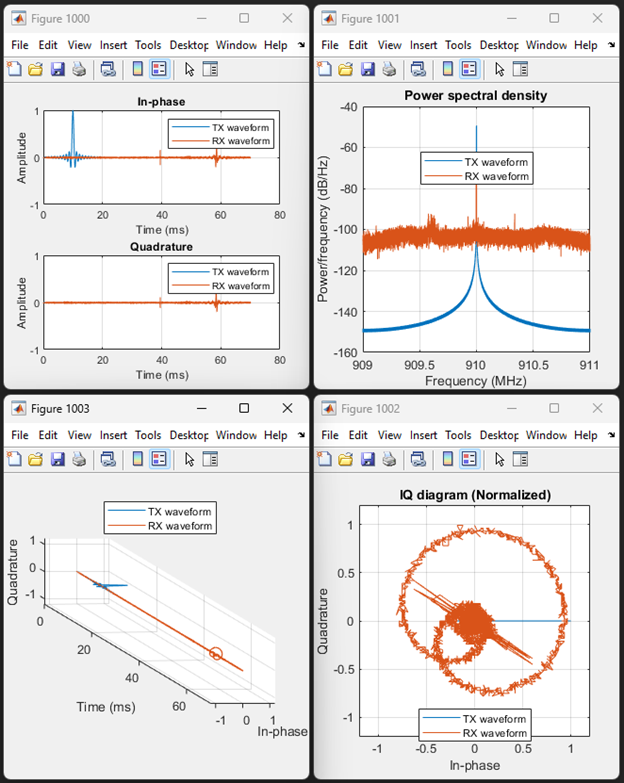
\includegraphics[width=\linewidth]{CA3_1_d.png}

\subsubsection*{Discussion}
Interestingly, the IQ data does not exhibit repeating sinusoids but forms a peculiarly shaped object in 2D space. The PSD shows a single spike at \(910 \text{ MHz}\), which aligns with the carrier frequency \(f_c\).

\subsubsection*{Theoretical vs. Practical Bandwidth}
The observed spike at \(f_c\) validates the unique behavior of the sinc message when used in a DSB-SC AM modulation scheme. While the theoretical bandwidth for the sinc signal is \(4 \text{ kHz}\), the experimental observations offer a single concentrated frequency component, making it an anomaly worth investigating further.



\section*{Conclusions}
This report covered different modulation schemes, each explored both theoretically and practically. MATLAB simulations were found to be in dis-agreement with theoretical calculations.

\end{document}
